% Chapter Template


\chapter{Results and Discussion}

\label{Chapter6:Results}

%----------------------------------------------------------------------------------------
% Transfer learning
% effect of loss function
% effect of camera intrinsic 
% effect of Hyper parameter
% Effect of recreating holes.. 
 
 
%----------------------------------------------------------------------------------------
In this chapter we have evaluated your system and presented a comparative results  based on different experimental setup discussed in section \ref{Chapter5:Methodology}. We have categorized our experiments into 3 different sections as shown in the table below \ref{table:Results_main} to investigate in three difference areas. This table lists all the experiments carried out for this study on depth estimation. In the following sections we will be describing our results mentioned in the table and will be discussing about it in its respective sections.  We have 3 accuracy values based on different threshold namely (a1, a2, and a2) and two error metrics namely root mean square error (RMSE) and log\_10 error as mentioned in section. To give a overview of this result setup in this Chapter, in Section \ref{Chapter6:Influence_Structural_Char} we have experiments performed only on encoder block, in Section \ref{Chapter6:Transfer_Learning}  we made experiments with different configuration on decoder block and finally in Section \ref{Chapter6:Hole_Regeneration} we evaluate the performance of holes regeneration idea. 

\bgroup
\def\arraystretch{1.35}%  1 is the default, change whatever you need
\begin{table}[h]
\begin{tabular}{p{0.05\linewidth}p{0.3\linewidth}p{0.1\linewidth}p{0.1\linewidth}p{0.08\linewidth}p{0.08\linewidth}p{0.07\linewidth}}
\hline
\textbf{\#} & \textbf{Model} & \multicolumn{3}{l}{\textbf{Accuracy}} & \multicolumn{2}{l}{\textbf{Error}} \\ \cline{3-7} 
                    &                        & \textbf{a1}       & \textbf{a2}       & \textbf{a3}      & \textbf{RMSE}         & \textbf{log\_10}      \\ \hline\hline
\multicolumn{7}{l}{\textbf{\texttt{Influence Of Structural Characteristics} (Section \ref{Chapter6:Influence_Structural_Char})}}                                            \\ \hline
E1                 &  A1  & 0.22         & 0.43          &  0.61       & 0.34            &   \textbf{0.01}           \\ \hline
E2                  & A2  &   \textbf{0.60}  & \textbf{0.859} & \textbf{0.93}      &  \textbf{0.19}          &0.11              \\ \hline 
\multicolumn{7}{l}{\textbf{\texttt{Influence Of Different Environment Specific Models} (Section \ref{Chapter6:Transfer_Learning})}}                                                                   \\ \hline
{E3}                  & {A2\_Holes} (N+S)              & \textbf{0.39}   & \textbf{0.58}   & \textbf{0.65}  & \textbf{0.27}      & \textbf{1.70}       \\ \hline
{E4}                  & {A2\_Holes} (S) & 0.33   & 0.55   & 0.63  & 0.34      & 1.78       \\ \hline
\multicolumn{7}{l}{\textbf{\texttt{Holes Regeneration} (Section \ref{Chapter6:Hole_Regeneration})}}                                                       \\ \hline
{E5}                  & {A2\_NoHoles}            & \textbf{0.98}   & \textbf{0.98}   & \textbf{0.98}  & \textbf{0.10}       & \textbf{0.18}        \\ \hline
{E6}                  & {A2\_Holes}              & 0.39   & 0.58   & 0.65  & 0.27      & 1.70       \\ \hline
\end{tabular}

\caption{This table list all the results of experimental configuration performed. (N+S) denotes that model trained on NYU\_v2 and SD\_v2, where as (S) denotes model trained on SD\_v2. Best scores are highlighted in bold text in their respective categories.}
\label{table:Results_main}
\end{table}
\egroup

Experiments \textbf{E1} and \textbf{E2} where performed to understand the importance of structural dependency of depth maps and to test our proposed model against the state of the art system. In experiments \textbf{E3} and \textbf{E4} we validate the influence of different environment and task based model influence in different systems also we can understand camera intrinsic properties over data from structure sensor and lastly by this we can also see the influence of transfer learning even when trained on different dataset with different feature properties. Experiments \textbf{E5} and \textbf{E6} was carried out to study behaviour of probabilistic distribution over the invalid pixel which we call it as holes, this leads us to answer the question of efficient way for depth estimation.

 
% Please add the following required packages to your document preamble:
% \usepackage{multirow}


\section{Influence of Structural Characteristics}
 \begin{figure}[h]
\settoheight{\tempdima}{\includegraphics[width=.32\linewidth]{example-image-a}}%
\centering\begin{tabular}{@{}c@{ }c@{ }c@{ }c@{}}
&\textbf{RGB} & \textbf{Truth} & \textbf{Predicted} \\
\rowname{E1 (a)}&
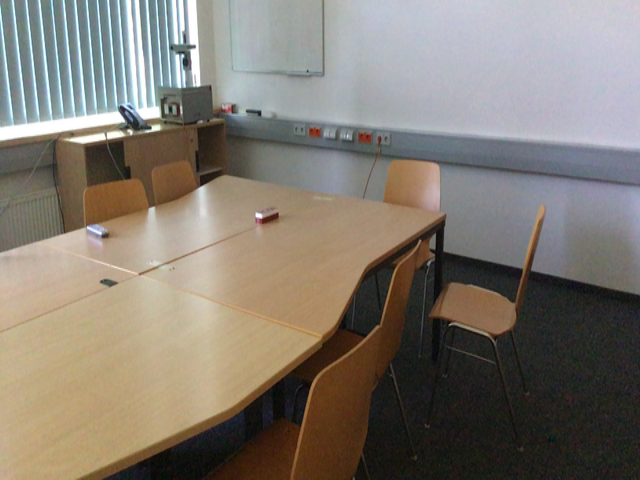
\includegraphics[width=.3\linewidth]{Figures/results/s1_a1/u0RAW_RGB.png}&
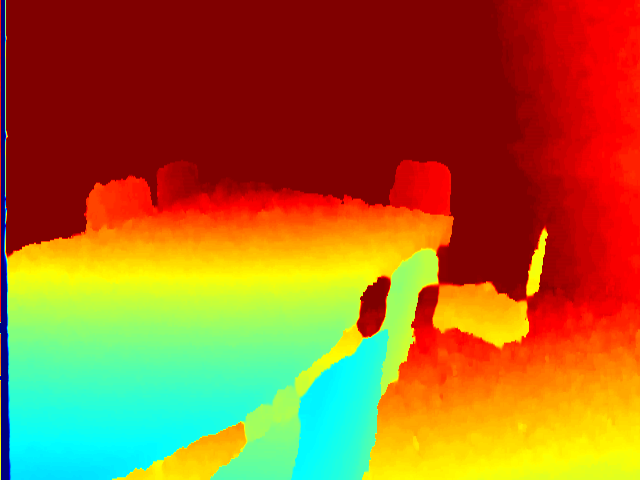
\includegraphics[width=.3\linewidth]{Figures/results/s1_a1/u0Truth.png}&
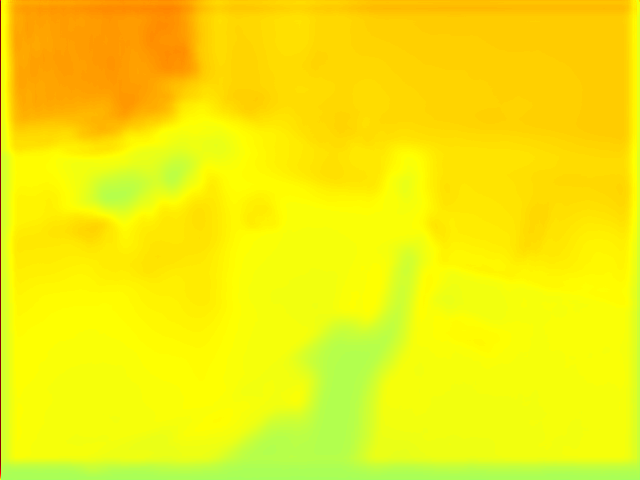
\includegraphics[width=.3\linewidth]{Figures/results/s1_a1/u0Predicted.png}\\[-1ex]
\rowname{E2 (b)}&
\includegraphics[width=.3\linewidth]{Figures/results/s1_a1/0RAW_RGB.png}&
\includegraphics[width=.3\linewidth]{Figures/results/s1_a1/0Truth.png}&
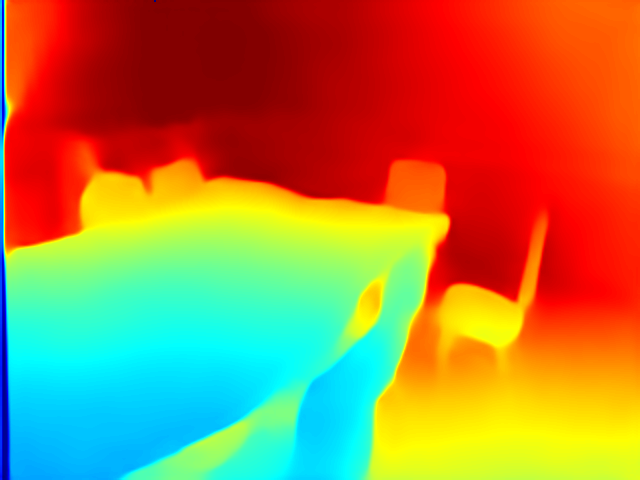
\includegraphics[width=.3\linewidth]{Figures/results/s1_a1/0Predicted.png}\\[-1ex]
\end{tabular}
\caption{\textbf{Influence of Structural Characteristics:} All the \textbf{E3} methods are in different  }%
\label{fig:results_E1_E2}
\end{figure}

\label{Chapter6:Influence_Structural_Char}
In this section we have investigated the Influence of Structural Characteristics of a pre-trained network backbone. \textbf{E1 - A1} model has no previously trained weights whereas \textbf{E2- A2} model has DenseNet backbone with pre trained weights only for the encoder part, which means, by evaluating \textbf{E1 - A1} against \textbf{E2 - A2} we can find out wheather the pre-trained backbone encoder model can have a influence over our results. One main significant different is in the decoder block, \textbf{A2} model is not trained on ImageNet as we discussed earlier in Section \ref{Chapter3:RelatedWork_NNModel} which implies the \textbf{A2} encoder has learnt Structural Characteristics feature from RBG images. Therefor we evaluate this influence of such pre-trained backbone. Therefore we train both the models with same SD\_v1 dataset with the train, validation and test set split of 80\%, 10\%  and 10\% respectively. Note that in \textbf{E2 - A2} case, we train only the decoder part. From the result in table \ref{table:Results_main} we see that the model performs gives a accuracy \textbf{a1} of only \textbf{0.22} which is 22 \% when compared with \textbf{A2} accuracy of \textbf{0.60}. Also the RMSE error is also high in \textbf{E1 - A1} compared to \textbf{E2 - A2}. Similarly the output from both the model in fig. \ref{fig:results_E3_E4} also shows  \textbf{E1 - A1} failed to perform. Important factor to notice is that, there were several layer parameters and hyper parameters where changed and tested before reaching the current \textbf{E1 - A2}. Due to the poor performance we did not document every step of model tuning of \textbf{E1 - A1} 

Observation: On a positive note for \textbf{E1 - A1} there are two things to be noted. First,  \textbf{E1 - A1} model can learn some structure characters as seen in the predicted image in fig. \ref{fig:results_E3_E4} \textbf{E1(a)} we notice that the chair could be identified to be closer than the wall behind. Second, we noticed that training and prediction is relatively  faster than \textbf{E2 - A2} model which means smaller network can give faster results. On the negative  side performance is very poor. 
Therefore, it is very clear that \textbf{E2 - A2} with DenseNet backbone outperforms \textbf{E1 - A1}. Since the accuracy of \textbf{E1 - A1} was extremely poor we believe that this is an effect of less data available for training, which gave us an motivation for SD\_v2  dataset to generate more data. Thus we believe for further experiments choosing \textbf{A2} model over \textbf{A1} would be beneficial. Which leads us to the second step of this study which is to answer, if we can train the network to reproduce the holes in the similar fashion to Structure Sensor. And we have a better working model \textbf{A2} but still not the best. Since as we see in Fig. \ref{fig:results_E1_E2} the sooth edges around the objects in the predicted frame. 
 


 

 \section{Influence of Different Environment Specific Models}
 \label{Chapter6:Transfer_Learning}
Second investigation the influence of different model which was developed for different environment and specific task. In this method we input depth image for the network was with holes, still keeping the primary objective in this second stage of experimental process of finding optimal model for the best results irrespective of what type of feature is given as input. In order to find the best working model, From the previous investigation we understood the impact of pre-trained backbone (encoder) in our case which is DenseNet, in this experiment we two different configuration changes only on decoder part by keeping the encoder unchanged. Initially in first experiment \textbf{E3 - A2\_Holes(N+S)}  we trained our decoder part with two datasets one from kinect sonsor (NYU\_v2) and Structure sensor (SD\_v2)and in the second experiment \textbf{E4 - A2\_Holes(S)} we only with Structure sensor (SD\_v2) dataset. By this we can study the effects and influence different camera properties in our results there by achieving optimal model for our task.

The results from the table \ref{table:Results_main} we notice that all the three accuracy of \textbf{E3 - A2\_Holes(N+S)} is higher than \textbf{E4 - A2\_Holes(S)} similarly both the error is also lower for \textbf{E3 - A2\_Holes(N+S)} which means \textbf{E3 - A2\_Holes(N+S)} perform better than  \textbf{E4 - A2\_Holes(S)}. But when we compare difference of these five metrics individually, we find that there are only small difference. For instance lets us consider RMSE, \textbf{E3 - A2\_Holes(N+S)} has error rate of \textbf{0.27} while \textbf{E4 - A2\_Holes(S)} error rate is \textbf{0.34} with difference \textbf{0.07}. In the same way for accuracy \textbf{a1}, the accuracy difference between both the configurations where only \textbf{0.06}, for \textbf{a2} is \textbf{0.03} and for \textbf{a3} is just \textbf{0.02}. 

But when we compare the resultant depth maps from these two experimental configurations, visually the difference are higher with respect to precision at the object boundaries which can be seen in the Fig.\ref{fig:results_E3_E4}  where \textbf{E3 (a) - E3(c)} represented the resultant output from \textbf{E3 - A2\_Holes(N+S)} and similarly  \textbf{E4 (a) - E4(c)} represented the output from \textbf{E4 - A2\_Holes(S)}. We notice two significant difference, first a blurred effect at object edges for the model trained only on SD\_v2 dataset, where as we get refined edges with \textbf{E4 - A2\_Holes(S)}. Secondly, we observe that our model \textbf{E3 - A2\_Holes(N+S)} has learnt the holes. What is more interesting is as we see in the Fig. \ref{fig:results_E3_E4} \textbf{E3 (b)} model can learn even the complex environment which is comprised of many pole looking structures (legs of chairs in a classroom environment).

Oservation: As we have seen that our \textbf{A2} model when trained with both dataset performs better than when trained on one dataset alone. On a positive note, we see that data from Kinect sensor has improved our results. On the other hand, when we consider the size of SD\_v2 compared with NVU\_v2, SD\_v2 is relatively small. So it is difficult to study and conclude the effect of camera properties. On the other hand the, another way to understand this effect we need a model which was only trained on NYU\_v2 and compare against our current model which is retrained with SD\_v2 dataset, since the Alhashim et. al. model was not trained no depth images with holes this would be a unfair comparison. Thus we perform another test in the following Section \ref{Chapter6:ComapreS-F-A} to validate the influence of camera properties on different environment. But with this test, we can say that NYU\_v2 dataset has a significant impact in our result.

 
 \begin{figure} [!]
\settoheight{\tempdima}{\includegraphics[width=.32\linewidth]{example-image-a}}%
\centering\begin{tabular}{@{}c@{ }c@{ }c@{ }c@{}}
&\textbf{RGB} & \textbf{Truth} & \textbf{Predicted} \\
\rowname{E3 (a)}&
\includegraphics[width=.3\linewidth]{Figures/results/s2_Holes/0RAW_RGB.png}&
\includegraphics[width=.3\linewidth]{Figures/results/s2_Holes/0Truth.png}&
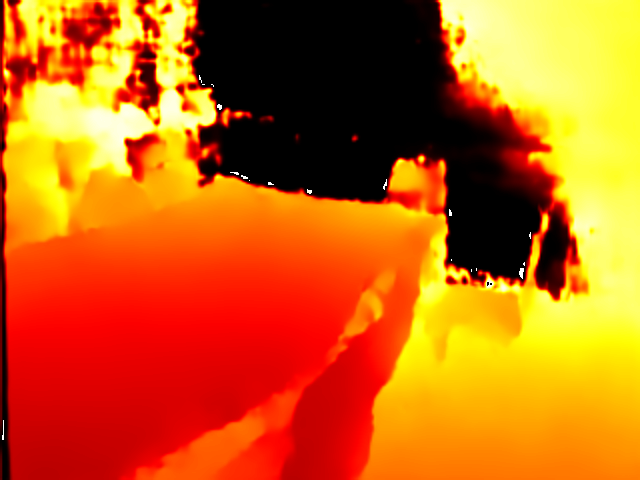
\includegraphics[width=.3\linewidth]{Figures/results/s2_Holes/0Predicted.png}\\[-1ex]
\rowname{E3 (b)}&
\includegraphics[width=.3\linewidth]{Figures/results/s2_Holes/1RAW_RGB.png}&
\includegraphics[width=.3\linewidth]{Figures/results/s2_Holes/1Truth.png}&
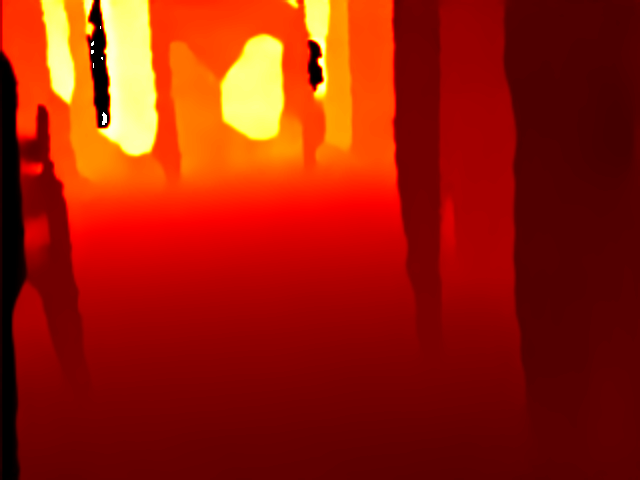
\includegraphics[width=.3\linewidth]{Figures/results/s2_Holes/1Predicted.png}\\[-1ex]
\rowname{E3 (c)}&
\includegraphics[width=.3\linewidth]{Figures/results/s2_Holes/2RAW_RGB.png}&
\includegraphics[width=.3\linewidth]{Figures/results/s2_Holes/2Truth.png}&
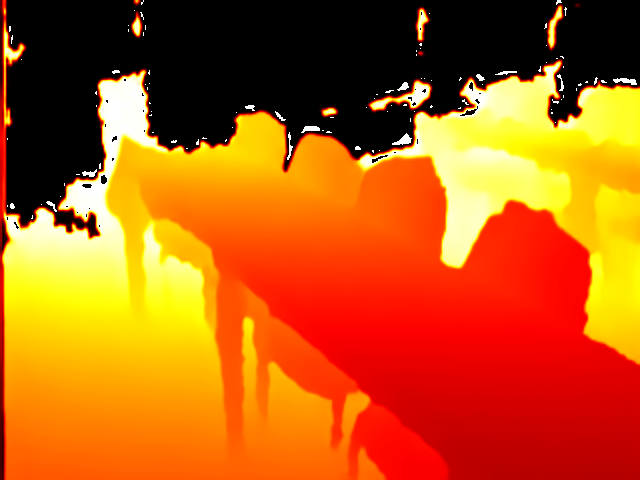
\includegraphics[width=.3\linewidth]{Figures/results/s2_Holes/2Predicted.png}\\[-1ex]
\rowname{E4 (a)}&
\includegraphics[width=.3\linewidth]{Figures/results/s3_noNyu/0RAW_RGB.png}&
\includegraphics[width=.3\linewidth]{Figures/results/s3_noNyu/0Truth.png}&
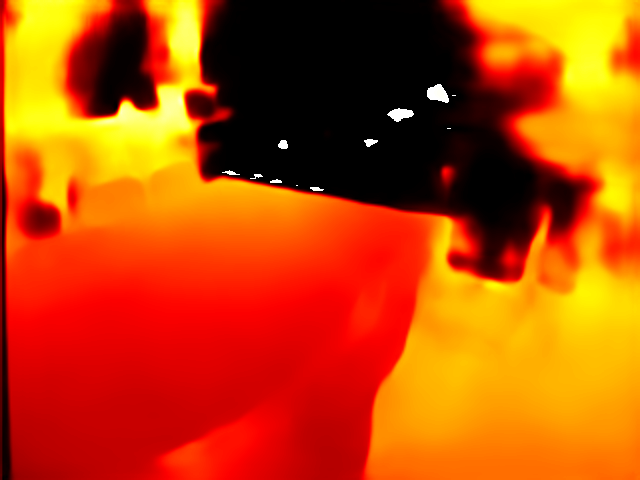
\includegraphics[width=.3\linewidth]{Figures/results/s3_noNyu/0Predicted.png}\\[-1ex]
\rowname{E4 (b)}&
\includegraphics[width=.3\linewidth]{Figures/results/s3_noNyu/1RAW_RGB.png}&
\includegraphics[width=.3\linewidth]{Figures/results/s3_noNyu/1Truth.png}&
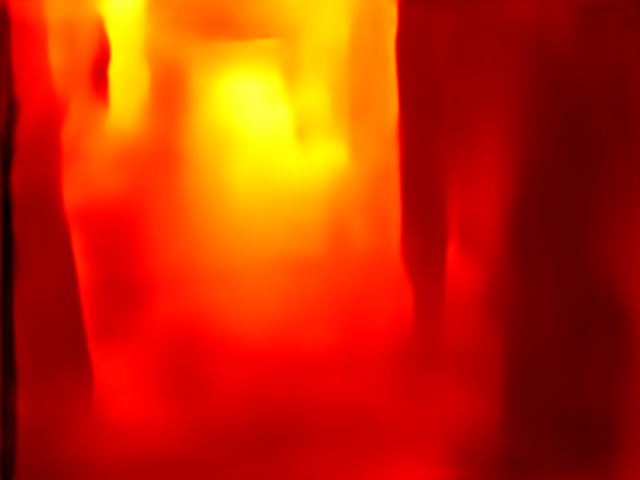
\includegraphics[width=.3\linewidth]{Figures/results/s3_noNyu/1Predicted.png}\\[-1ex]
\rowname{E4 (c)}&
\includegraphics[width=.3\linewidth]{Figures/results/s3_noNyu/2RAW_RGB.png}&
\includegraphics[width=.3\linewidth]{Figures/results/s3_noNyu/2Truth.png}&
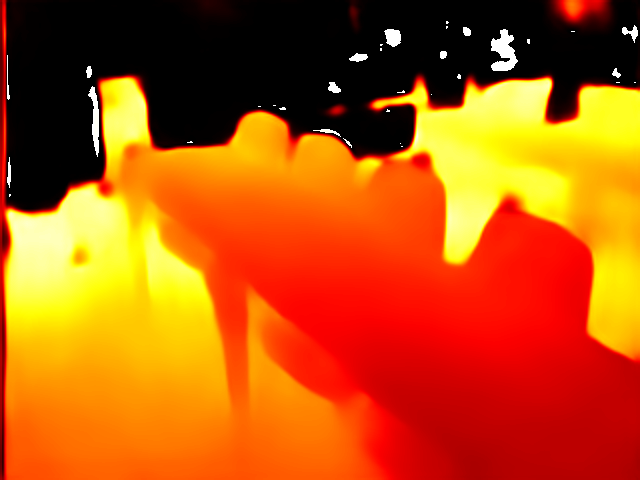
\includegraphics[width=.3\linewidth]{Figures/results/s3_noNyu/2Predicted.png}\\[-1ex]
\end{tabular}
\caption{\textbf{Investigation on hole regeneration method:} All the \textbf{E3} methods are in different  }%
\label{fig:results_E3_E4}
\end{figure}



 Also we wanted to study the influence of effects of a probabilistic distribution (in other words neural network's output is a distribution of probable values ranging from 0.0 to 1.0 on a image level) over this regenerating holes. As described in Section \ref{Chapter4:Dataset}, in order to have a holes recreated we mapped all the dead value or no pixel region as zero.


 \section{Hole Regeneration}
 \label{Chapter6:Hole_Regeneration}


Further more to improve the results for estimation of depth maps for 3D reconstruction, we wanted to validate whether re generation of hole can give us better results. Therefore we have two methods of pre-possessing carried out with two different input feature type, one with holes and another without holes. We tested the performance of \textbf{A2\_Holes} against the \textbf{A2\_NoHoles} models. In Fig. \ref{fig:results_S2} (a) - (c) we see that there a good reconstruction of the depth map were all the holes were interpolated to its neighboring pixel.  Fig. \ref{fig:results_S2} \textbf{(d) - (f)}  corresponds to the model with the holes as a input to the network. As we see in Fig \ref{fig:results_S2}, we compare \textbf{E5} and \textbf{E6}. We have used two different color maps for \textbf{E5} and \textbf{E6}. This is because in \textbf{E4} we wanted to highlight the difference between holes which were mapped to zero and the closest region in an image. 


From the table \ref{table:Results_main} we notice that the on an average the model \textbf{E5 - A2\_NoHoles} performs better. When RMSE is taken into consideration we can clearly see that \textbf{E5 - A2\_NoHoles} performs better with the RMSE of \textbf{0.10} which is \textbf{0.17} lower than the \textbf{E4 - A2\_Holes} with RMSE of \textbf{0.27}. Visually we see that both the models have very good performance. We also see the depth prediction of the complex image like in Fig. \ref{fig:results_S2} \textbf{E5(b)} and  \textbf{E6(b)} can learn the depth features and the predicted image resembles to ground truth. Thus we have a model \textbf{E5 - A2\_NoHoles} which can perform good with average accuracy of \textbf{0.98}. But when we notice our accuracy a1, a2 and a3 for both the models we see the difference of results when compared with each other, for a1 the difference in \textbf{0.59} similarly \textbf{0.40} and \textbf{0.33} for a2 and a3 respectively. These difference are high even though we notice in the Fig. \ref{fig:results_S2} we have visually good prediction. This motivated us to investigated further to find the reason behind such hugh difference in the accuracy and error. Hence we visualized the predicted imaged from both the model and mapped in a 3D space using the method proposed by \cite{Zhou2018} and the results are shown in Fig. \ref{fig:3drecon}. We notice that in \ref{fig:3drecon} \textbf{(a)}, there are many intermediate pixel predicted in between zero value (here zeros are holes) till the next nearest non-holes pixel. Also in this approach intermediate pixels are most prone to be predicted in front of the object (in between zero and the next possible neighboring pixel with non-hole value) in 3D space which is not desirable and the for removal of such artifacts, we need careful post processing techniques. It turns out that these intermediate pixels cannot be seen from the perspective of the camera, thus the Fig. \ref{fig:3drecon} \textbf{(a)} shown is rotated for better visualization of such intermediate pixels. Where as we do not see such effects in \textbf{E5 - A2\_NoHoles} rather we see a wall like structure mapped to the highest possible value. This is the most common phenomenon which we wanted to eradicate. Therefore we believe that, this is one of the factors responsible for lower accuracy rate for the \textbf{E6 A2\_Hole} model. 

 \begin{figure}[!]
\settoheight{\tempdima}{\includegraphics[width=.32\linewidth]{example-image-a}}%
\centering\begin{tabular}{c@{ }c@{ }c@{ }}
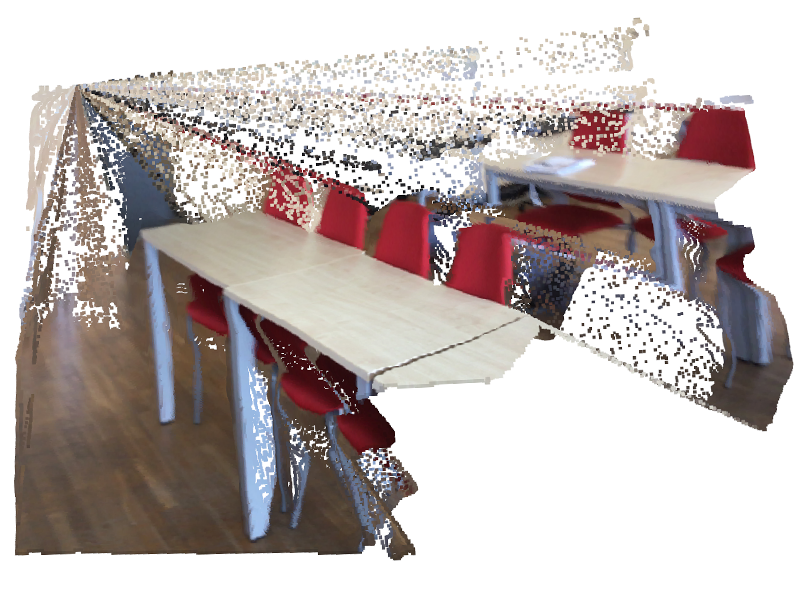
\includegraphics[width=.5\linewidth]{Figures/results/3D/holes001.png}&
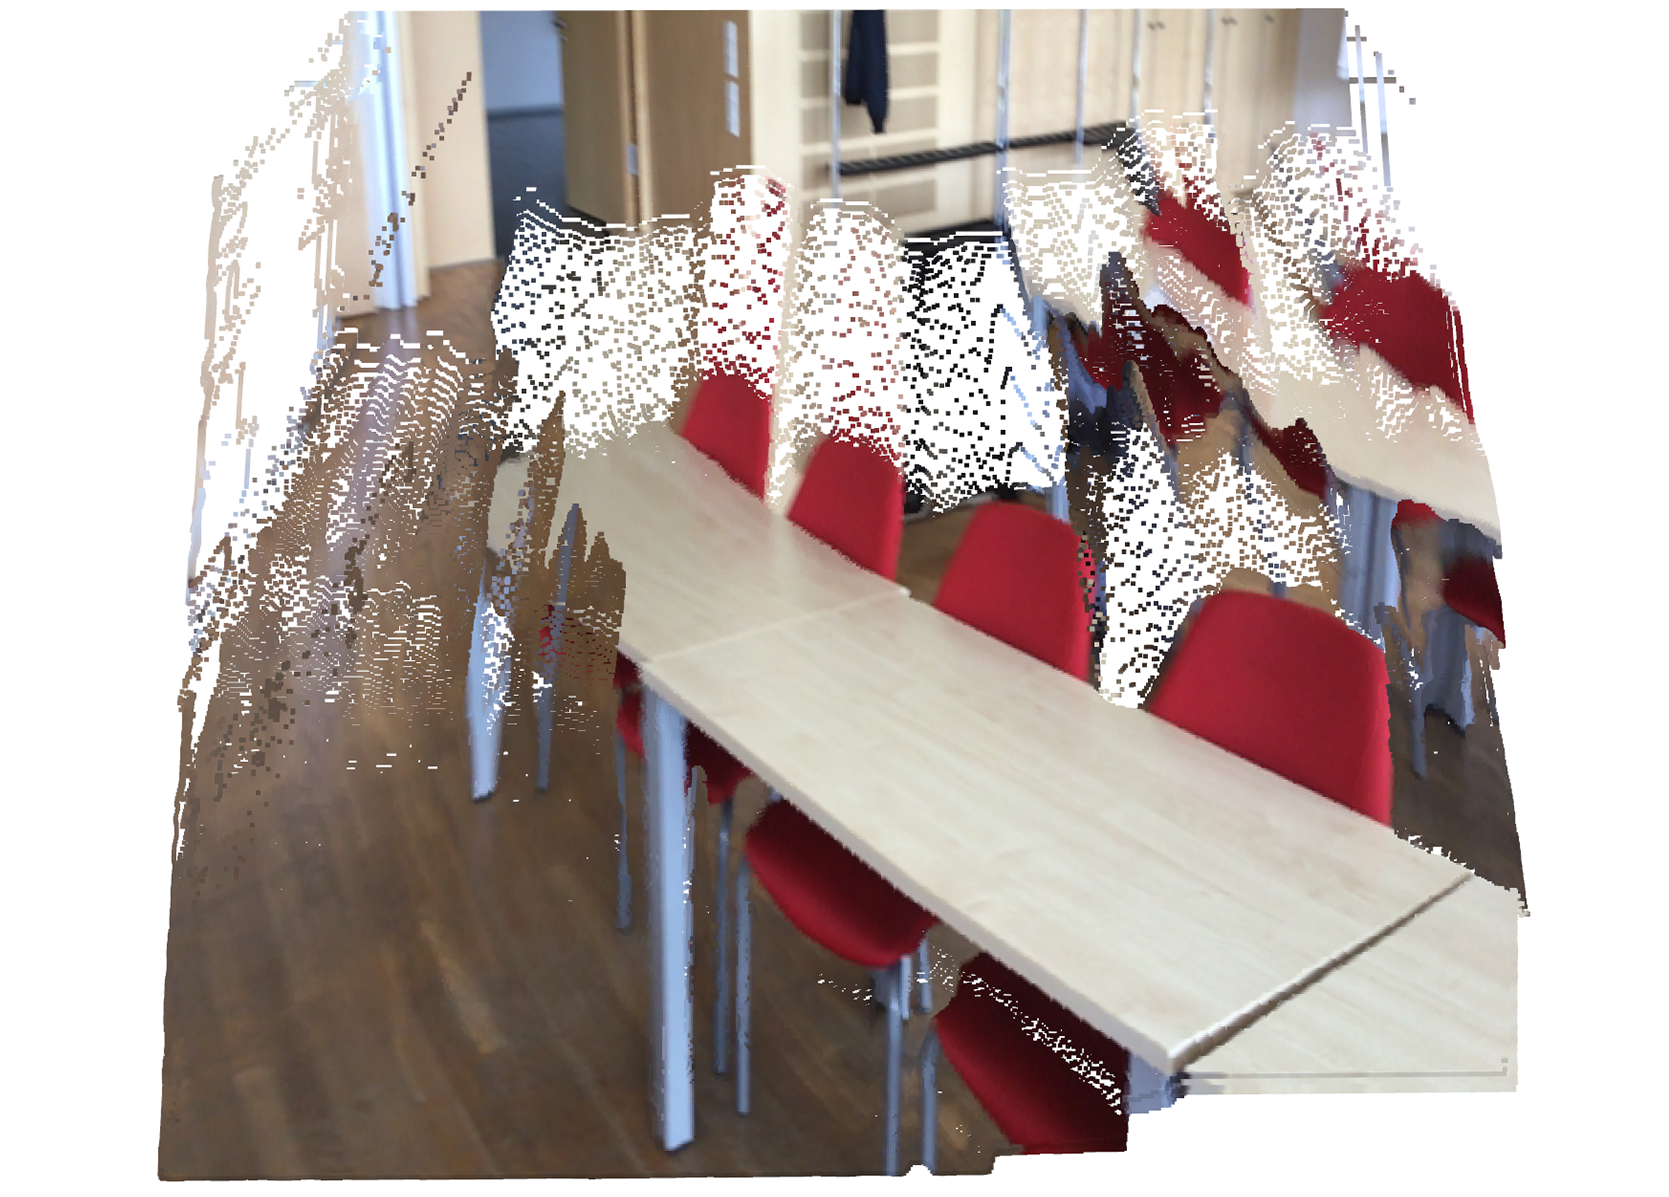
\includegraphics[width=.5\linewidth]{Figures/results/3D/noholes002.png}\\[-1ex]
\end{tabular}
\caption{3D Visualization of depth map}
\label{fig:3drecon}
\end{figure}

Observation: Since we discussed about the two factors. One with the perspective of accuracy, which is as high as \textbf{0.98} and another with respective of practical application for 3D reconstruction. Both the approach has a good depth prediction visually but for the application where the object dimensions are crucial approach with \textbf{E6\_NoHoles} will be beneficial since the intermediate pixels are comparatively less. 
Therefore we see that given an input with holes the model can learn the holes from the given monocular image. But it results into intermediate pixel effect, which we believe makes the 3D reconstruction of a scene more difficult and demands further post processing techniques. We also stated that one of the reason for training on dataset with holes is to remove the wall effect. We see that network can learn but the one of the other motivation to try this approach was to eliminate the wall effect of depth maps  for the pixel farther than the distance limit, one approach for this solution could be taking a threshold just before the highest pixels. This solves the problem of having wall in out 3D reconstruction scene.\\


\begin{figure} [!]
\settoheight{\tempdima}{\includegraphics[width=.32\linewidth]{example-image-a}}%
\centering\begin{tabular}{@{}c@{ }c@{ }c@{ }c@{}}
&\textbf{RGB} & \textbf{Truth} & \textbf{Predicted} \\
\rowname{E5 (a)}&
\includegraphics[width=.3\linewidth]{Figures/results/s2_NoHoles/0RAW_RGB.png}&
\includegraphics[width=.3\linewidth]{Figures/results/s2_NoHoles/0Truth.png}&
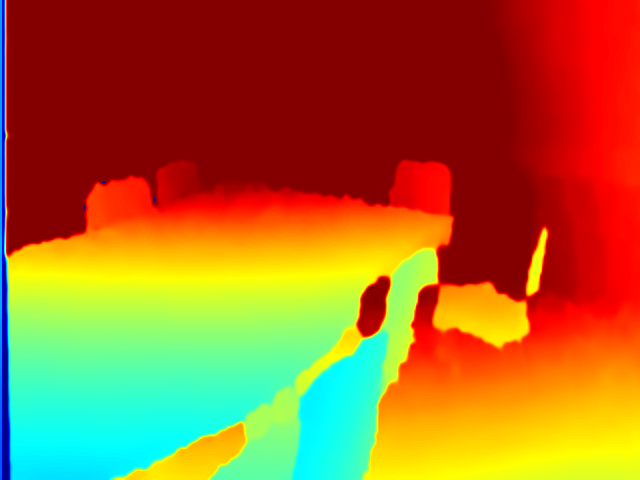
\includegraphics[width=.3\linewidth]{Figures/results/s2_NoHoles/0Predicted.png}\\[-1ex]
\rowname{E5 (b)}&
\includegraphics[width=.3\linewidth]{Figures/results/s2_NoHoles/1RAW_RGB.png}&
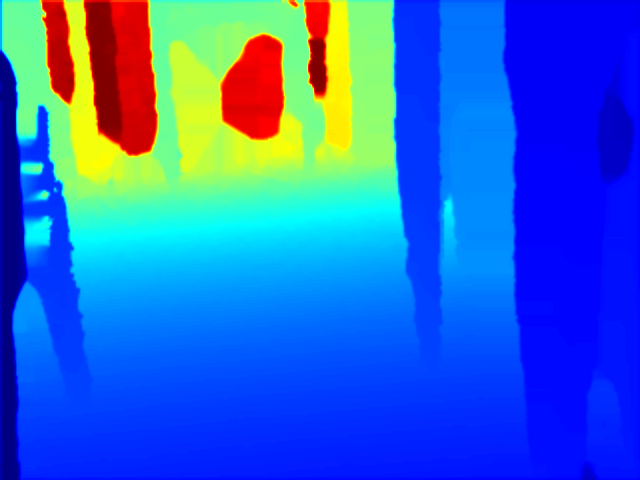
\includegraphics[width=.3\linewidth]{Figures/results/s2_NoHoles/1Truth.png}&
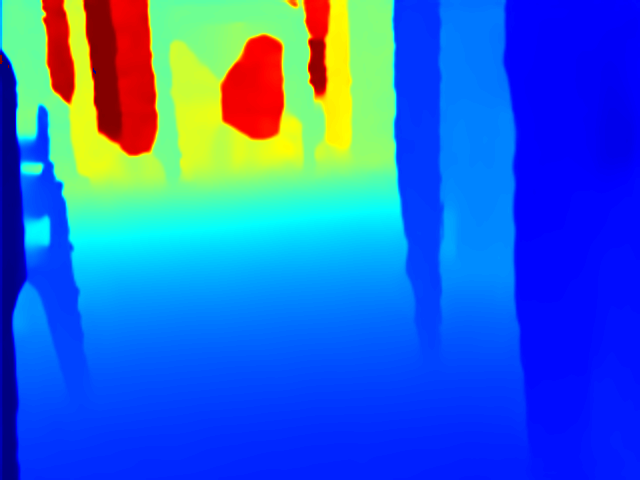
\includegraphics[width=.3\linewidth]{Figures/results/s2_NoHoles/1Predicted.png}\\[-1ex]
\rowname{E5 (c)}&
\includegraphics[width=.3\linewidth]{Figures/results/s2_NoHoles/2RAW_RGB.png}&
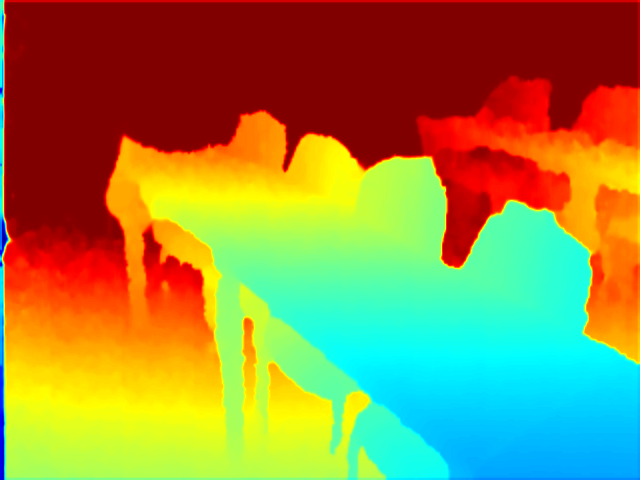
\includegraphics[width=.3\linewidth]{Figures/results/s2_NoHoles/2Truth.png}&
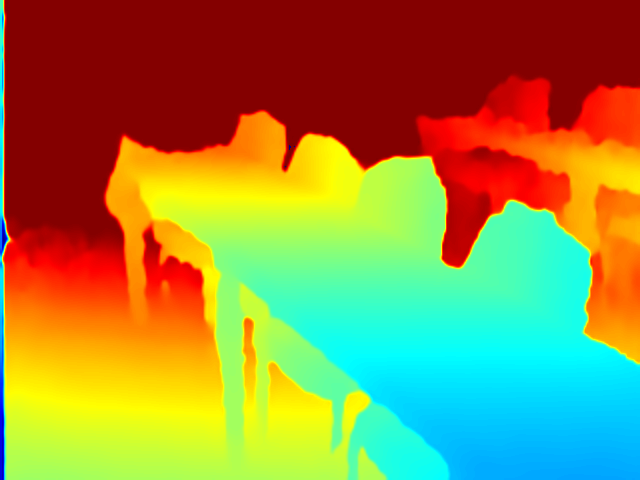
\includegraphics[width=.3\linewidth]{Figures/results/s2_NoHoles/2Predicted.png}\\[-1ex]
\rowname{E6 (a)}&
\includegraphics[width=.3\linewidth]{Figures/results/s2_Holes/0RAW_RGB.png}&
\includegraphics[width=.3\linewidth]{Figures/results/s2_Holes/0Truth.png}&
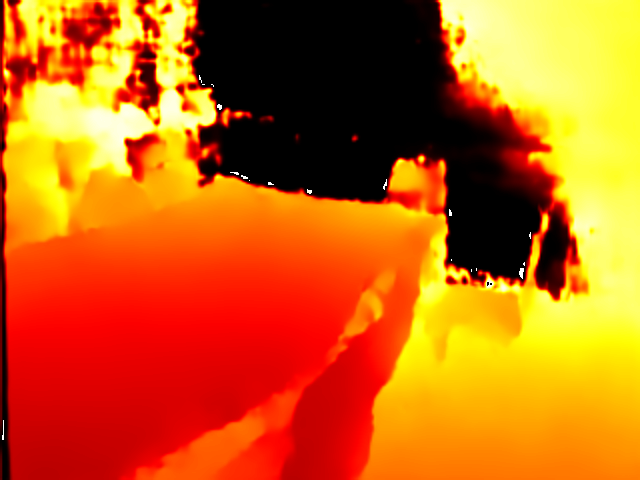
\includegraphics[width=.3\linewidth]{Figures/results/s2_Holes/0Predicted.png}\\[-1ex]
\rowname{E6 (b)}&
\includegraphics[width=.3\linewidth]{Figures/results/s2_Holes/1RAW_RGB.png}&
\includegraphics[width=.3\linewidth]{Figures/results/s2_Holes/1Truth.png}&
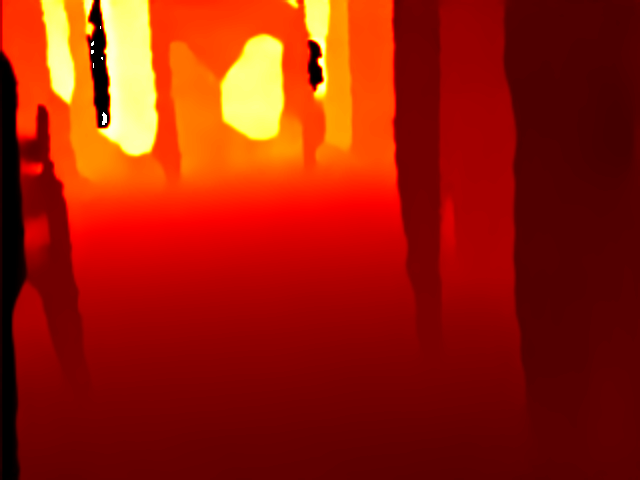
\includegraphics[width=.3\linewidth]{Figures/results/s2_Holes/1Predicted.png}\\[-1ex]
\rowname{E6 (c)}&
\includegraphics[width=.3\linewidth]{Figures/results/s2_Holes/2RAW_RGB.png}&
\includegraphics[width=.3\linewidth]{Figures/results/s2_Holes/2Truth.png}&
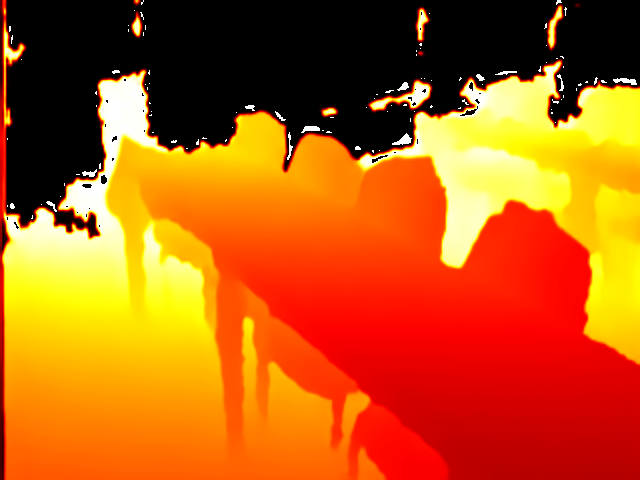
\includegraphics[width=.3\linewidth]{Figures/results/s2_Holes/2Predicted.png}\\[-1ex]
\end{tabular}
\caption{\textbf{Investigation on hole regeneration method:} All the \textbf{E3} methods are in different  }%
\label{fig:results_S2}
\end{figure}



This leads us to an conclusion that for 3D reconstruction task, interpolating of pixel is a better approach than making than network learn to predict holes because of intermediate pixel effect. But on the other hand for for estimation of depth of a frame level for distance measurement both the approach. Hence with the accuracy of \textbf{0.98} on \textbf{E5 A2\_NoHoles} and a good 2D and 3D visual analysis we believe this is our best model configuration sfter series of experiments.




\newpage
\section{Comparison With Baseline System}
 \label{Chapter6:ComapreS-F-A}


From the above result, we have achieved reasonably good performing model which can learn to predict depth images which is trained to fit the structure sensor environment. For the final test for this study we would also like to compare current best working model configuration \textbf{E5 - A2\_NoHoles} with the current state of the art proposed by Alhashim et. al. \cite{Alhashim2018}. Our motivation for this evaluation to validate if our model fits the required environment (Structure Sensor and IPad) for specific task for indoor 3D reconstruction. This can be achieved by comparing with Alhashim et. al. model which was trained on different environment. This will also eventually gives us an better understanding for various qeustion. First, as discussed in Section \ref{Chapter6:Transfer_Learning} where we where unable to give a definite conclusion regarding effects of difference camera properties, with such experiment we aim to get a better understating of such effect. Second, we can justify the need for the reason for generating environment based and task based dataset (SD) to fit our model. For both the methods listed in table \ref{table:Results_SFA} we used SD test set which was described in Section \ref{Chapter4:DatasetForsplits-i} for both the methods. 

\begin{table}[h]
\centering
\begin{tabular}{p{0.3\linewidth}p{0.1\linewidth}p{0.1\linewidth}p{0.08\linewidth}p{0.08\linewidth}p{0.07\linewidth}} \hline
\textbf{Methods} & \multicolumn{2}{l}{\textbf{Accuracy}} & {\textbf{Error}} \\ \cline{2-6} 
    &  a1& a2  & a3    & RMSE & log\_10   \\ \hline \hline
\textbf{Alhashim} \cite{Alhashim2018}    &  0.39 & 0.65   &  0.82  & \textbf{0.23}   &   0.16  \\ \hline

\textbf{Our (E2 - A2\_NoHoles)}     &   \textbf{0.89} & \textbf{0.98} & \textbf{0.99}   & 0.39  & \textbf{0.043}  \\ \hline

\end{tabular}
\caption{Comparison with state of the art}
\label{table:Results_SFA}
\end{table} 


We in general notice that there is significance difference in accuracy between both the models from the above table \ref{table:Results_SFA}. When considered accuracy \textbf{Our} model performs better. For example, accuracy \textbf{a1} the difference is about \textbf{0.50}, similarly for \textbf{0.33}, \textbf{0.17} for \textbf{a2} and \textbf{a3} respectively. Meanwhile \textbf{Alhashim} has lower \textbf{RMSE} error which contractics the accuracy score. But we have lower error score \textbf{log\_{10}} which supports the accuracy score. For this it is also important to have a visual evaluation. As we see in Fig. \ref{fig:results_SFA} there is a significant difference between both the models, The model trained on NYU\_v2 dataset with Kinect Sensor dataset can learn the structural characteristic and also the depth but the difference lies in the scale of these depth maps. Visually, we see for model trained on only Kinect Sensor dataset the prediction of closer depth appears to be much closer than the ground truth. Which clearly shows that there is some influence of different model tuned for specific environment and task.

Observation: Thus we believe that it is difficult for a model to generalize on different environment and task. For this, proper and careful tuning of the model has to be done to in order to get state of the art performance for specific tasks. In our case since both the models are developed for different tasks, it is difficult to compare and based on general performance but \textbf{Our} model is more suitable for the designed environment. Hence this also answers the importance of generation of dataset. Added to this we can also say we see some influence of different camera properties with respect to the scale (actual distance) but with these tests alone we cannot specifically find the specific parameter influence and also it is out of the scope this study. 



 \begin{figure}[h]
\settoheight{\tempdima}{\includegraphics[width=.32\linewidth]{example-image-a}}%
\centering\begin{tabular}{@{}c@{ }c@{ }c@{ }c@{}}
&\textbf{RGB} & \textbf{Truth} & \textbf{Predicted} \\
\rowname{Alhashim}&
\includegraphics[width=.3\linewidth]{Figures/results/s2_NoHoles/0RAW_RGB.png}&
\includegraphics[width=.3\linewidth]{Figures/results/s2_NoHoles/0Truth.png}&
\includegraphics[width=.3\linewidth]{Figures/results/sfa/0Pred.png}\\[-1ex]
\rowname{Our}&
\includegraphics[width=.3\linewidth]{Figures/results/s2_NoHoles/0RAW_RGB.png}&
\includegraphics[width=.3\linewidth]{Figures/results/s2_NoHoles/0Truth.png}&
\includegraphics[width=.3\linewidth]{Figures/results/s2_NoHoles/0Predicted.png}\\[-1ex]
\rowname{Alhashim}&
\includegraphics[width=.3\linewidth]{Figures/results/s2_NoHoles/1RAW_RGB.png}&
\includegraphics[width=.3\linewidth]{Figures/results/s2_NoHoles/1Truth.png}&
\includegraphics[width=.3\linewidth]{Figures/results/sfa/1Pred.png}\\[-1ex]
\rowname{Our}&
\includegraphics[width=.3\linewidth]{Figures/results/s2_NoHoles/1RAW_RGB.png}&
\includegraphics[width=.3\linewidth]{Figures/results/s2_NoHoles/1Truth.png}&
\includegraphics[width=.3\linewidth]{Figures/results/s2_NoHoles/1Predicted.png}\\[-1ex]
\rowname{Alhashim}&
\includegraphics[width=.3\linewidth]{Figures/results/s2_NoHoles/2RAW_RGB.png}&
\includegraphics[width=.3\linewidth]{Figures/results/s2_NoHoles/2Truth.png}&
\includegraphics[width=.3\linewidth]{Figures/results/sfa/2Pred.png}\\[-1ex]
\rowname{Our}&
\includegraphics[width=.3\linewidth]{Figures/results/s2_NoHoles/2RAW_RGB.png}&
\includegraphics[width=.3\linewidth]{Figures/results/s2_NoHoles/2Truth.png}&
\includegraphics[width=.3\linewidth]{Figures/results/s2_NoHoles/2Predicted.png}\\[-1ex]
\end{tabular}
\caption{\textbf{Influence of Structural Characteristics:} All the \textbf{E3} methods are in different  }%
\label{fig:results_SFA}
\end{figure}

In summary, after series of various testing with the different models and configurations we achieved the best performing model which is \textbf{E2 - A2\_NoHoles} (re trained model \textbf{A2} with  interpolating configuration )


\newpage

